\documentclass{article}

\usepackage{graphicx}
\usepackage{tikz}
\usepackage{tikzsymbols}
\usetikzlibrary{calc,patterns,shapes.geometric}
\pagestyle{empty}
\usepackage[margin=0pt]{geometry}
\geometry{papersize={14in,12in}}

\def\centerarc[#1](#2)(#3:#4:#5){\draw[#1] ($(#2)+({#5*cos(#3)},{#5*sin(#3)})$) arc (#3:#4:#5);}

\begin{document}
	\begin{figure}
		\centering
		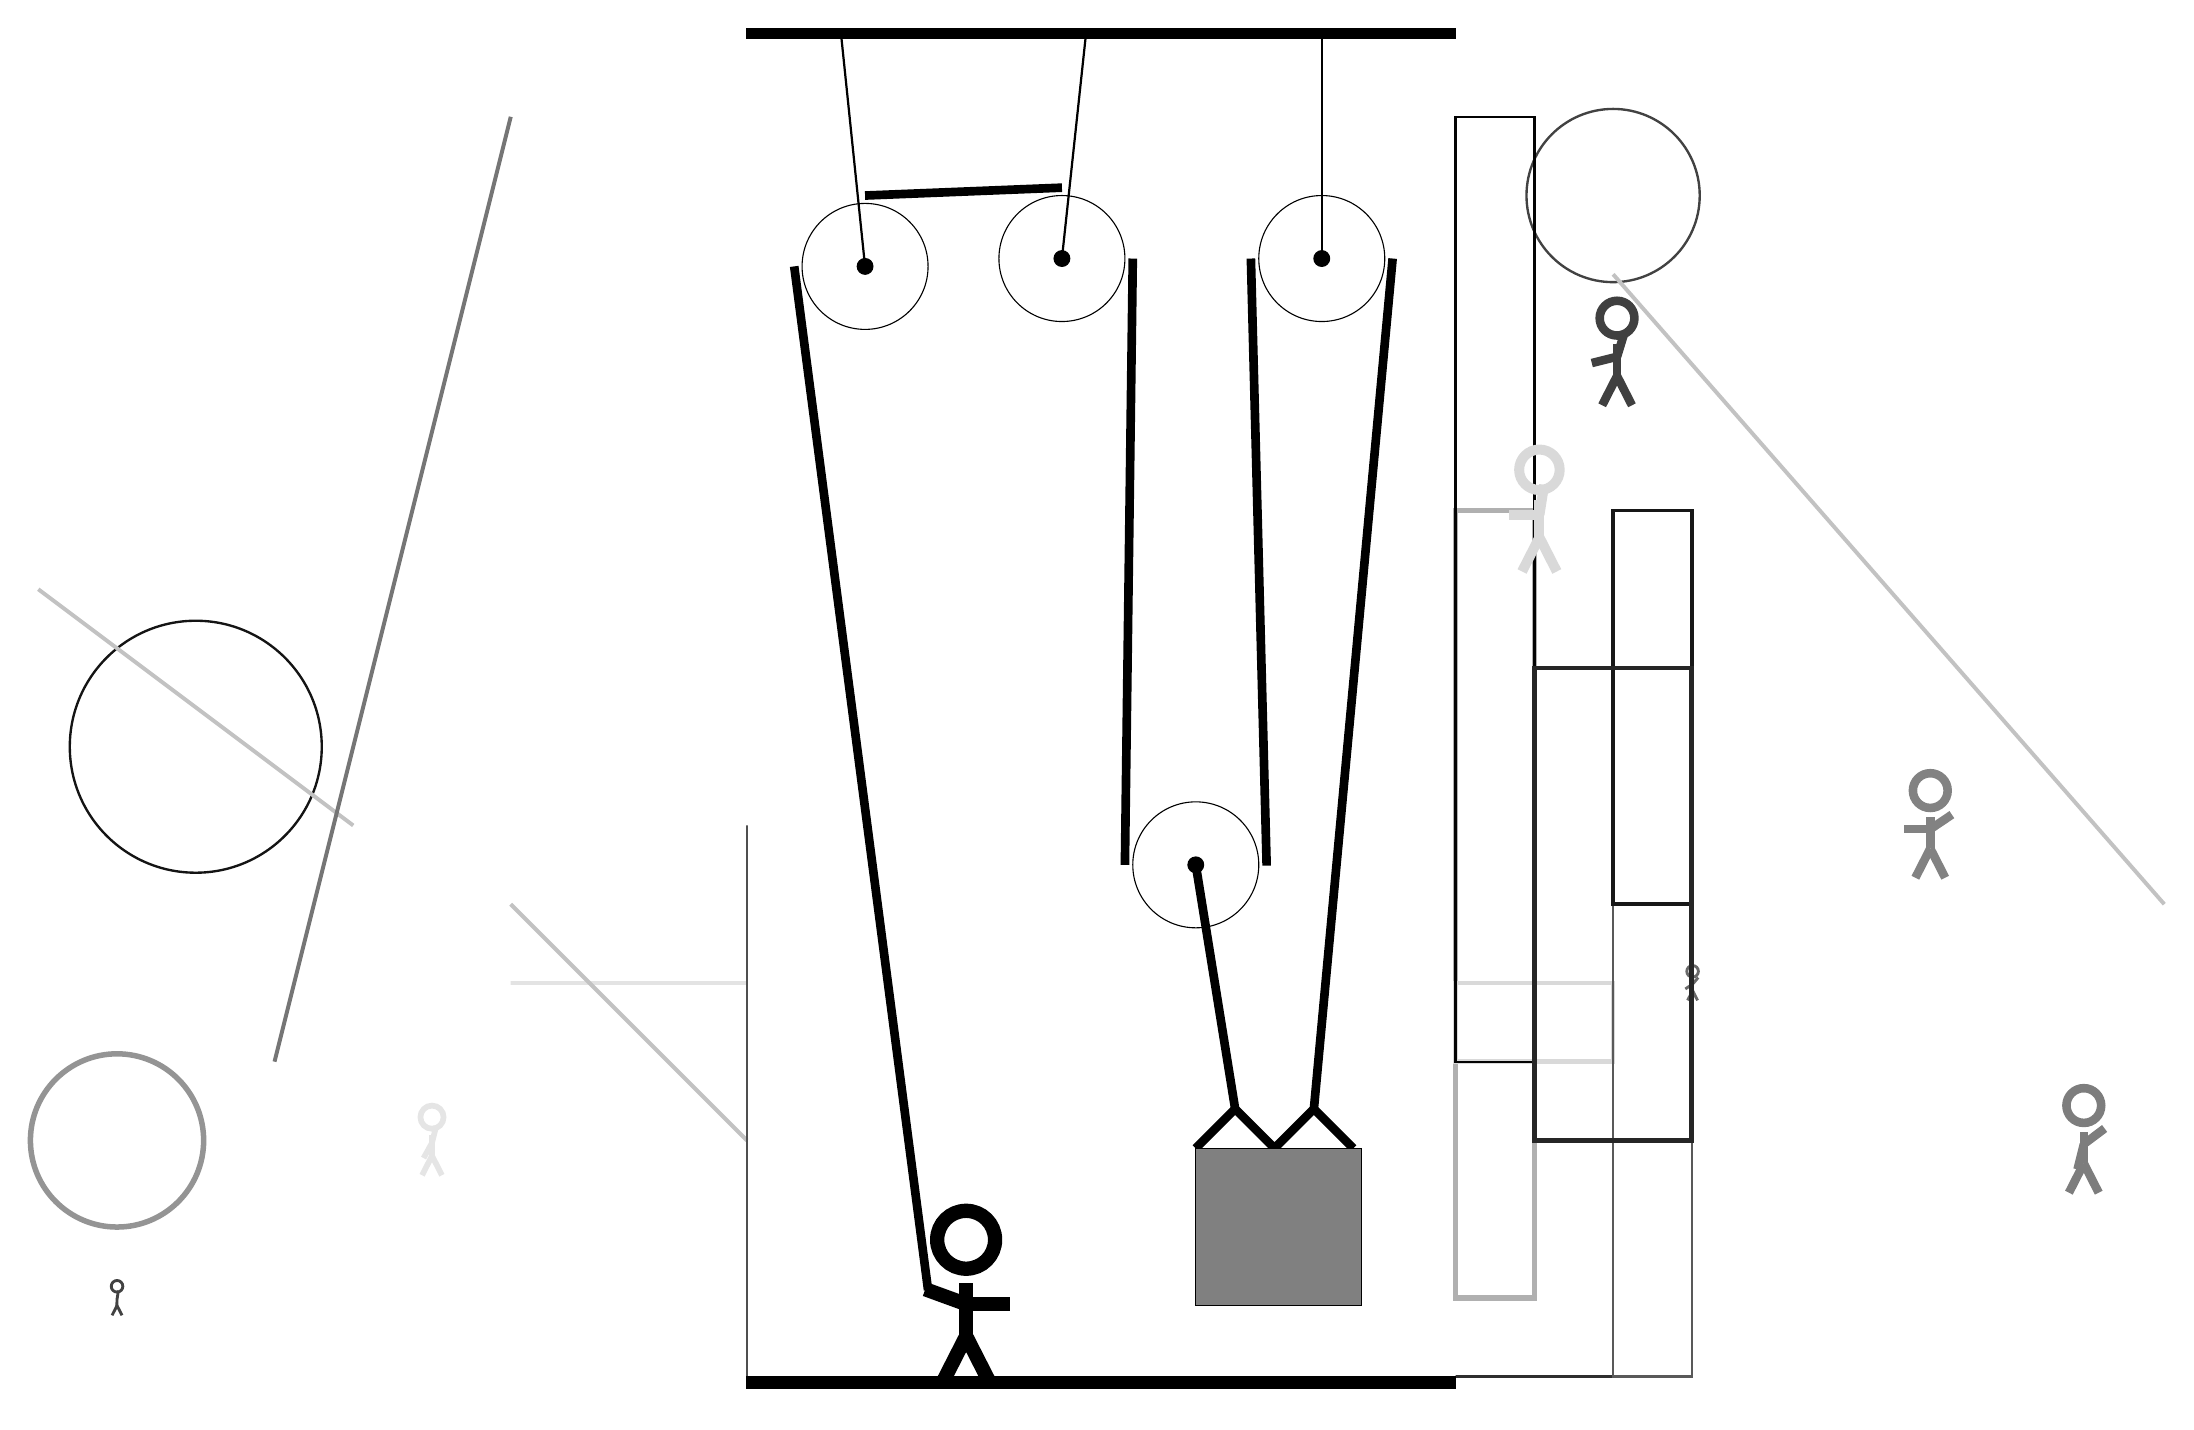
\begin{tikzpicture}
			%%%%% START %%%%%
			
			\draw[fill=black] (-3, 14) rectangle (6, 14.125);
			
			\draw (1, 11.2) circle (0.8);
			\draw[fill=black] (1, 11.2) circle (0.1);
			\draw[thick] (1, 11.2) -- (1.3, 14);
			
			\draw (4.3, 11.2) circle (0.8);
			\draw[fill=black] (4.3, 11.2) circle (0.1);
			\draw[thick] (4.3, 11.2) -- (4.3, 14);
			
			\draw (2.7, 3.5) circle (0.8);
			\draw[fill=black] (2.7, 3.5) circle (0.1);
			
			\draw[line width=1.1mm]  (2.7, -0.1) -- (3.2, 0.4) -- (3.7, -0.1) -- (4.2, 0.4) -- (4.7, -0.1);
			\draw[fill=black!50] (2.7, -0.1) rectangle (4.8, -2.1);
			
			\draw (-1.5, 11.1) circle (0.8);
			\draw[fill=black] (-1.5, 11.1) circle (0.1);
			\draw[thick] (-1.5, 11.1) -- (-1.8, 14);
			
			\draw[line width=1.1mm](-0.7, -1.9) --  (-2.4, 11.1);
			\centerarc[line width=1.1mm](-1.5, 11.1)(90:180:0.9);
			\draw[line width=1.1mm](-1.5, 12.0) -- (1, 12.1);
			\centerarc[line width=1.1mm](1, 11.2)(0:90:0.9);
			\draw[line width=1.1mm](1.9, 11.2) -- (1.8, 3.5);
			\centerarc[line width=1.1mm](2.7, 3.5)(180:370:0.9);
			\draw[line width=1.1mm] (3.6, 3.49) -- (3.4, 11.2);
			\centerarc[line width=1.1mm](4.3, 11.2)(0:180:0.9);
			\draw[line width=1.1mm](4.2, 0.4) -- (5.2, 11.2);
			\draw[line width=1.1mm] (3.2, 0.4) -- (2.7, 3.5);
			
			\node[line width=0.7mm, color=black!59] at (9, 2) {\Strichmaxerl[2][33][50]};
			
			\node[line width=0.7mm, color=black!75] at (8, 10) {\Strichmaxerl[6][14][73]};
			\node[line width=0.7mm, color=black!74] at (-11, -2) {\Strichmaxerl[2][88][81]};
			\draw [line width=0.7mm, color=black!42](-11, 0) circle (1.1);
			
			\draw[line width=0.4mm, color=black!82] (8, -3) rectangle (6, -3);
			\node[line width=0.2mm, color=black!51] at (14, 0) {\Strichmaxerl[6][76][37]};
			\draw[line width=0.5mm, color=black!11] (-3, 2) rectangle (-6, 2);
			
			\draw[line width=0.7mm, color=black!31] (7, -2) rectangle (6, 8);
			\node[line width=0.3mm, color=black!49] at (12, 4) {\Strichmaxerl[6][0][34]};
			\node[line width=0.2mm, color=black!10] at (-7, 0) {\Strichmaxerl[4][61][76]};
			\draw[line width=0.6mm, color=black!15] (8, 1) rectangle (6, 2);
			
			\draw [line width=0.3mm, color=black!92](-10, 5) circle (1.6);
			\draw [line width=0.3mm, color=black!74](8, 12) circle (1.1);
			\draw[line width=0.5mm, color=black!24](-3, 0) -- (-6, 3);
			\draw[line width=0.3mm, color=black!99] (6, 1) rectangle (7, 13);
			\draw[line width=0.2mm, color=black!69] (-3, -3) rectangle (-3, 4);
			\draw[line width=0.5mm, color=black!24](-8, 4) -- (-12, 7);
			\draw[line width=0.3mm, color=black!65] (8, -3) rectangle (9, 8);
			\draw [line width=0.3mm, color=black!91](-7, -1) circle (0.0);
			\node[line width=0.7mm, color=black!15] at (7, 8) {\Strichmaxerl[7][0][81]};
			\draw[line width=0.5mm, color=black!91] (8, 8) rectangle (9, 3);
			
			\draw[line width=0.6mm, color=black!85] (7, 6) rectangle (9, 0);
			
			\draw[line width=0.5mm, color=black!54](-6, 13) -- (-9, 1);
			\draw[line width=0.5mm, color=black!24](8, 11) -- (15, 3);
			
			\node at (-0.2, -2) {\Strichmaxerl[10][-20][0]};
			
			\draw[fill=black] (-3, -3) rectangle (6, -3.15);
			
			%%%%% END %%%%%
		\end{tikzpicture}
	\end{figure}	
\end{document}